\paragraph{Pre-registration.} We ran \NumProtocols{} protocols (v5--v13). Each was committed to a public repository
before any score on its test data existed. Each fixes:
\begin{itemize}
  \item networks, splits and seeded test panels;
  \item model recipes;
  \item endpoints, statistics and pass rules.
\end{itemize}
Every endpoint is reported, failures included (Table~\ref{tab:all-endpoints}). Model changes were selected on data
already used by an earlier protocol, by rules written into the next protocol, and then confirmed on networks never
used before (v9, v10).

\paragraph{Networks.} The thirteen networks are listed in Table~\ref{tab:networks}.
\begin{itemize}
  \item \textbf{Traffic:} speed on METR-LA and PEMS-BAY, flow on PeMS03 and PeMS08.
  \item \textbf{Indoor climate:} Intel Lab temperature.
  \item \textbf{Air quality:} PM$_{2.5}$ in China and the UK; NO$_2$ in the UK.
  \item \textbf{Weather:} temperature and pressure from the German weather service.
  \item \textbf{Hydrology:} river discharge from three US states.
\end{itemize}
Seven networks have test periods in April--September 2026, after the release of TabPFN v2 (January 2025).
TabPFN-3.5 was released on September 9, 2026, near the end of these periods. We cannot rule out that its training
data include some of these public records; that would favour TabPFN-3.5, not our models.

\paragraph{Episodes and conditions.} Each test episode predicts one held-out sensor from its 11 neighbours. It has
48 labelled support rows from the same time window, a day to a week. Metrics are computed on 48 query rows, under
three conditions:
\begin{itemize}
  \item the natural mask, ``all sensors'';
  \item $+3$ further inputs dropped at random;
  \item $+6$ further inputs dropped at random.
\end{itemize}

\paragraph{Baselines.}
\begin{itemize}
  \item \textbf{TabPFN v2}~\citep{hollmann2025tabpfnv2}, in context with 8 estimators. Missing inputs are passed as
  NaN.
  \item \textbf{TabPFN-3.5}~\citep{jaeger2026tabpfn35}, the default model of the \texttt{tabpfn} package since
  September 2026, run exactly like TabPFN v2 (8 estimators, its default) on the four 2026 networks (protocol v13).
  \item \textbf{PFN-L.} A plain cell-token transformer with UPT's backbone, size and training budget, but only the
  free head: the matched-scale ablation. It is trained with the same SF pipeline and test-time ensemble as UPT.
  \item \textbf{Neural processes:} TNP-D~\citep{nguyen2022tnp} and CNP~\citep{garnelo2018cnp}, trained on the same
  prior and fine-tuned with the same recipe.
  \item \textbf{Deep kriging:} an IGNNK-style inductive kriging model~\citep{wu2021ignnk} trained on each network's
  source period. Its \emph{calibrated} variant is recalibrated by an affine map on each episode's support, the
  stronger of the two.
  \item \textbf{Closed forms:} FA-Gaussian (UPT's anchor) and EM-Gaussian (simple kriging).
  \item \textbf{Tabular baselines:} LightGBM and multiple imputation (Appendix~\ref{app:results}).
\end{itemize}
UPT-SF is UPT-L with the SF pipeline, the CRPS-augmented objective and the 8-member test-time ensemble, chosen by the
pre-registered rule of protocol v10.

\subsection{Results}
\label{sec:results}

\begin{table}[t]\centering\small
\caption{\textbf{Pre-registered endpoints on the four fresh 2026 networks.} NLL gain in nats (baseline $-$ ours; positive favours the first method), paired 95\% interval clustered by network-window; \checkmark: pass (gain $\geq 0.01$ and lower bound $>0$). Protocols v12 and v13 (TabPFN-3.5, September 2026) test the mechanism and a newer foundation model on the same networks after v11; v14 tests the variant selected on development networks, and $^\dagger$ marks a secondary comparison.}
\label{tab:fresh}
\setlength{\tabcolsep}{3pt}
\begin{tabular}{llccc}
\toprule
Protocol & Comparison & All inputs & 3 dropped & 6 dropped \\
\midrule
v11 & UPT-SF$\oplus$TabPFN vs TabPFN v2 & +0.17 [+0.14, +0.20] \checkmark & +0.24 [+0.20, +0.29] \checkmark & +0.60 [+0.49, +0.72] \checkmark \\
v11 & UPT-SF$\oplus$TabPFN vs UPT-SF alone & +0.91 [+0.76, +1.06] \checkmark & -- & -- \\
v13 & UPT-SF$\oplus$TabPFN-3.5 vs TabPFN-3.5 & +0.04 [+0.03, +0.06] \checkmark & +0.03 [+0.01, +0.04] \checkmark & +0.03 [+0.01, +0.04] \checkmark \\
v13 & UPT-SF$\oplus$TabPFN-3.5 vs UPT-SF alone & +1.33 [+1.13, +1.53] \checkmark & -- & -- \\
v14 & UPT site$\,\otimes\,$TabPFN-3.5 vs TabPFN-3.5 & +0.01 [-0.01, +0.03] $\times$ & -0.01 [-0.06, +0.04] $\times$ & +0.01 [-0.02, +0.05] $\times$ \\
v14$^\dagger$ & UPT site$\,\otimes\,$TabPFN-3.5 vs UPT-SF$\oplus$TabPFN-3.5 & -0.03 [-0.05, -0.02] $\times$ & -0.04 [-0.08, +0.01] $\times$ & -0.01 [-0.04, +0.02] $\times$ \\
v12 & UPT-SF$\oplus$TabPFN vs PFN-L$\oplus$TabPFN & +0.12 [+0.08, +0.16] \checkmark & +0.12 [+0.08, +0.16] \checkmark & +0.09 [+0.05, +0.12] \checkmark \\
v12 & UPT-SF$\oplus$TabPFN vs FA$\oplus$TabPFN & +0.10 [+0.08, +0.12] \checkmark & +0.11 [+0.10, +0.13] \checkmark & +0.12 [+0.10, +0.13] \checkmark \\
v10 & UPT-SF alone vs TabPFN v2 & -0.75 [-0.93, -0.58] $\times$ & -0.63 [-0.81, -0.45] $\times$ & -0.21 [-0.44, +0.03] $\times$ \\
\bottomrule
\end{tabular}
\end{table}

\begin{figure}[t]
\centering
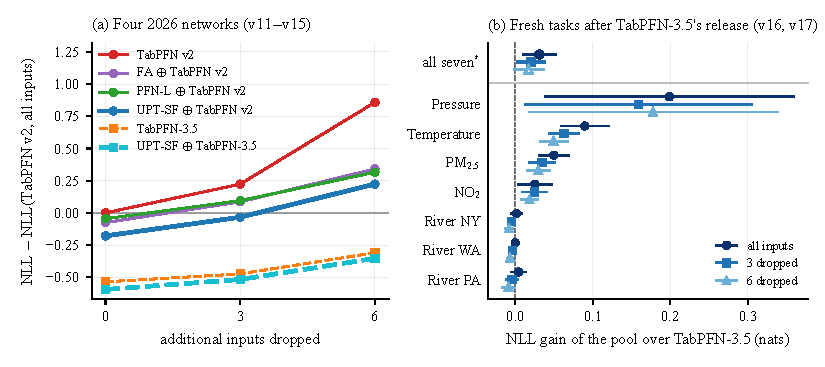
\includegraphics[width=\linewidth]{figures/pool_fresh.pdf}
\caption{\textbf{(a) Robustness to failing inputs} on the four 2026 networks: mean NLL relative to TabPFN v2 with all
inputs. TabPFN v2 degrades by 0.86 nats at six dropped inputs; pooling it with any partner helps, and UPT is the best
partner. TabPFN-3.5 (dashed) is far stronger and more robust; pooling it with UPT (v15 rule) still improves it at every
level. \textbf{(b) Fresh tasks recorded after TabPFN-3.5's release:} NLL gain of the frozen v15 pool over TabPFN-3.5 on
each network (95\% $t$-intervals over network-windows; descriptive) and on all seven pooled ($^*$the pre-registered
endpoints, 97.5\% intervals; open marker: the interval reaches zero).}
\label{fig:robust}
\end{figure}

\paragraph{UPT\,$\oplus$\,TabPFN on fresh 2026 data (protocols v11, v12).} Every pre-registered endpoint of the
pooled model passes (Table~\ref{tab:fresh}, pooled over \FreshEpisodes{} episodes on four networks).
\begin{itemize}
  \item \textbf{Against TabPFN v2,} the gain grows with the number of failed inputs: \XOne{} nats with all inputs,
  \XTwoThree{} with three dropped, \XTwoSix{} with six dropped.
  \item \textbf{On each network separately} the pool beats TabPFN v2 too: by 0.07--0.44 nats with all inputs and by
  0.16--1.69 with six dropped (Table~\ref{tab:pool}).
  \item \textbf{The stacking weights are interpretable.} With no test label, they place 72--83\% of the weight on
  TabPFN for the two river networks with all inputs, whose near-deterministic targets suit its sharp predictive. They place 68--97\%
  on UPT for pressure and PM$_{2.5}$, rising as inputs fail. With TabPFN-3.5 they track the two models' relative skill
  in the same way (Figure~\ref{fig:weights}).
\end{itemize}

\paragraph{Is it the partner or just pooling? (protocol v12).} Pooling TabPFN with any reasonable partner helps under
input failure: TabPFN alone loses 0.86 nats at six dropped inputs (Figure~\ref{fig:robust}a). The partner still
matters. With the same stacking rule, UPT is a better partner than:
\begin{itemize}
  \item the plain transformer of equal size and training: \YOneZero{} nats with all inputs, \YOneSix{} with six
  dropped;
  \item the closed-form lifted sites: \YTwoZero{} and \YTwoSix{}.
\end{itemize}
Both ingredients of UPT therefore contribute: the lifted sites beat the plain transformer, and the learning beats
the closed form. The largest margin is on the pressure network: UPT\,$\oplus$\,TabPFN scores $-0.60$ against $-0.12$
for PFN-L\,$\oplus$\,TabPFN.

\paragraph{The newest foundation model (protocols v13, v15).} TabPFN-3.5 (September 2026) is far stronger than
TabPFN v2 on these networks (by 0.3--1.3 nats) and degrades much less when inputs fail. The same pool, run unchanged
(v13), still improves it: \ZOne{} nats with all inputs, \ZTwoThree{} and \ZTwoSix{} with three and six dropped. On
pressure, UPT alone beats TabPFN-3.5 at every level ($-0.57$ vs $-0.47$ with all inputs), and UPT is a better partner
than a plain transformer by $+0.05$ to $+0.07$ nats. On the rivers, however, the pool lost 0.015--0.03 nats. With learning-curve-aware stacking (v15,
selected on development networks), the gains grow to \VOne{}, \VTwoThree{} and \VTwoSix{} nats, the pool beats the
v13 pool at every level (\VPoolZero{} with all inputs), and the river losses shrink by 75--95\%, to at most 0.008
nats (Figure~\ref{fig:crossfit}). The pre-registered claim that it is never worse than TabPFN-3.5 on any network fails narrowly: \VThreePass{} of
\VThreeN{} non-inferiority tests pass, the three failures being rivers with inputs dropped.

\paragraph{Fresh tests after TabPFN-3.5's release (protocols v16, v17).} The test periods of v13--v15 precede
TabPFN-3.5's release. We therefore froze the v15 rule and scored it once on new tasks: days after the release
(September 10 -- October 12) and 48 target sensors per network that no protocol had used. On the four v10 networks
(v16) the pool beats TabPFN-3.5 with all sensors (\FOne{} nats); with inputs dropped the gains (\FTwoThree{},
\FTwoSix{}) are as large as v15 predicted, but with 30 clusters their intervals reach zero. v17 added the three v9
networks and tested all \GEpisodes{} tasks (\GClusters{} clusters) at the 97.5\% level of a second look: the pool wins
with all sensors (\GOne{}) and with three dropped (\GTwoThree{}); with six dropped (\GTwoSix{}) the interval reaches
zero. Gains are large where UPT alone beats TabPFN-3.5 (pressure, temperature) and smaller on air quality; rivers tie
with all sensors and lose at most 0.009 nats with inputs dropped (Figures~\ref{fig:robust}b and~\ref{fig:fresh-curves}).

\paragraph{Beyond averaging fails confirmation (protocol v14).} A linear pool is never sharper than its sharper member
on a single query. Of the combinations that could be (UPT's predictive as inputs of TabPFN-3.5, TabPFN-3.5 on UPT's
residuals, the logarithmic pool $p\propto p_F^a\,\mathcal N(m_{\mathrm{UPT}},v_{\mathrm{UPT}})^b$), development
selected the logarithmic pool, which then failed every confirmatory endpoint (\ROne{}, \RTwoThree{}, \RTwoSix{}),
losing up to 0.12 nats on rivers: unlike the linear pool (Proposition~\ref{prop:pool}), it has no loss bound.

\begin{table}[t]\centering\small
\caption{\textbf{Mean test NLL (nats; lower is better)} with all sensors (left of the slash) and with six extra sensors dropped (right). Learned models: mean over three seeds. Best per row in bold. Networks recorded in 2026 are below the rule; the last four are protocol v10, never used before its endpoints were scored. On USGS NY the UPT-SF mean is dominated by 15 episodes with a constant support target (\S\ref{sec:results}).}
\label{tab:main}
\setlength{\tabcolsep}{3pt}
\begin{tabular}{lcccccc}
\toprule
Network & UPT-SF & PFN-L & TabPFN v2 & TNP-D & Krig.\ (cal.) & FA-Gauss. \\
\midrule
METR-LA & \textbf{-1.82}/\textbf{-1.60} & -1.48/-1.09 & -1.79/-1.21 & -1.37/-0.44 & -0.50/+0.30 & -0.15/-0.29 \\
PEMS-BAY & \textbf{-2.68}/\textbf{-2.34} & -2.42/-2.03 & -2.68/-2.06 & -2.11/-0.92 & -1.46/-0.57 & -0.94/-1.02 \\
Intel Lab & -0.95/\textbf{-0.02} & -0.32/+0.79 & \textbf{-1.30}/+2.36 & +0.03/+1.75 & +0.94/+2.72 & +0.49/+0.64 \\
PeMS03 & \textbf{-1.30}/\textbf{-1.00} & -1.03/-0.80 & -1.04/-0.04 & -0.93/-0.16 & -0.42/-0.34 & -0.57/-0.52 \\
PeMS08 & \textbf{-2.54}/\textbf{-2.12} & -1.12/-1.01 & -1.82/-0.62 & -1.07/-0.43 & -0.68/-0.94 & -1.28/-1.27 \\
China air & \textbf{-0.25}/\textbf{-0.03} & -0.12/+0.06 & -0.24/+0.92 & -0.05/+0.21 & +0.17/+0.51 & +0.27/+0.26 \\
\midrule
DWD temp. & \textbf{+1.02}/\textbf{+1.22} & +1.04/+1.25 & +1.32/+2.14 & +1.19/+1.62 & +1.39/+1.49 & +1.52/+1.45 \\
AURN NO$_2$ & \textbf{+0.22}/\textbf{+0.41} & +0.23/+0.44 & +0.30/+0.62 & +0.31/+0.55 & +0.37/+0.54 & +0.47/+0.51 \\
USGS PA & -2.62/-2.27 & -2.26/-1.97 & \textbf{-3.66}/\textbf{-2.72} & -1.82/-0.91 & -0.82/-0.37 & -0.86/-1.08 \\
USGS NY & +2024.7/+1305.6 & -1.56/-1.34 & \textbf{-3.63}/\textbf{-2.88} & -1.41/-0.75 & +85.3/+85.8 & -0.17/-0.26 \\
USGS WA & -3.31/-2.98 & -2.73/-2.47 & \textbf{-4.97}/\textbf{-4.41} & -2.51/-2.11 & -1.95/-1.78 & -2.22/-2.24 \\
DWD pressure & \textbf{-0.57}/\textbf{-0.22} & -0.01/+0.14 & -0.15/+1.46 & +0.09/+1.40 & +0.15/+0.65 & +0.07/+0.03 \\
AURN PM$_{2.5}$ & -0.40/\textbf{-0.21} & -0.27/-0.10 & \textbf{-0.43}/+0.07 & -0.21/+0.06 & -0.07/+0.08 & +0.13/+0.08 \\
\bottomrule
\end{tabular}
\end{table}

\paragraph{UPT alone across thirteen networks (protocols v6--v10; Table~\ref{tab:main}).} At matched size and
training, UPT has a lower mean NLL than the plain transformer on 12 of 13 networks at every sensor-loss level. It
beats TNP-D on all six v6/v7 networks (pre-registered v8: $+0.38$, $+0.53$, $+1.05$ nats at 0, 3, 6 dropped) and
calibrated deep kriging by more than one nat. Against TabPFN v2 alone it is better on 10 of 13 networks with six
inputs dropped ($+0.33$ nats pooled, descriptive) and on 8 of 13 with all inputs.

\paragraph{Failures.} We report all of them (Appendix~\ref{app:protocols}).
\begin{enumerate}
  \item \textbf{UPT alone loses to TabPFN v2 on the river networks} (v9, v10). The pre-registered pooled NLL tests of
  UPT alone against TabPFN on the 2026 networks fail. On rivers TabPFN's predictive is far sharper, at about the same
  RMSE; UPT's synthetic prior (five sensors, one factor) is far narrower than TabPFN's.
  \item \textbf{A degenerate case.} When all 48 support targets are identical (15 of 1{,}437 New York episodes),
  UPT's predictive collapses; this breaks v10's comparisons of UPT alone with the transformer, TNP-D and kriging.
  \item \textbf{With all inputs, TabPFN v2 alone remains better on 5 of 13 networks} (v6 P3, v9). Ablations from
  earlier protocols are in Appendix~\ref{app:protocols}.
\end{enumerate}

